\documentclass[10pt]{article}
\usepackage[pdftex]{graphicx}
\usepackage[utf8]{inputenc}
\usepackage{amsmath}
\usepackage{enumerate}
\usepackage{alltt}
\usepackage{float}
\usepackage{bbold}
\usepackage{caption}
\usepackage{subcaption}
\usepackage{subfig}
\restylefloat{table}
\usepackage{appendix}

\title{Symbolic Execution in Ruby\\
CMSC 631 Final Project}
\author{Elizabeth McNany and David Wasser}
\date{May 16, 2013}

\begin{document}
\maketitle

\begin{abstract}
Here is an abstract
\end{abstract}

\section{Introduction}
Security has become a major concern in application development in recent years.  Insecure software has been exploited and leveraged to steal large amount of money or information from various private and public organizations.  It has also been used to stop the operation of various websites or companies, resulting in large losses in revenue and damage to public image.\\

We are proposing an implementation of dynamic symbolic execution to help mitigate these vulnerabilities within Ruby applications.  This approach would allow developers to confirm that values are guaranteed to be within a specified acceptable range or that certain values are unaffected by other input values during the execution of the program.\\

Symbolic execution is a method of finding all possible outputs and paths of a program.  This is done by treating each variable as a symbolic variable that is a function of other variables in the program instead of a single value.  This allows a developer to confirm that a value will always be within a certain acceptable range, that a value will never influence another variable, or that a program will never execute certain code or run in an unintended way.  Symbolic execution will follow every single possible branch of a progra and run it to completion or failure.  Clearly, this approach can have a number of large problems resulting from complexity in the program and the exponential growth of execution paths at each branch.\\

Symbolic execution for security verification in Ruby software is nothing new \cite{rails}.  While it has been done before, we could not find one that followed our exact approach of implementing symbolic execution in Ruby to test for potential errors or assertion failures.\\

Our approach is to create a symbolic variable for a couple specified variables and then store this symbolic form along with the real value.  We will not follow every single path that is possible in the program, but will instead let it run as normal.  We will keep track of all operations done on the symbolic variables throughout the execution.  The user will also be able to add assertions, and as the program runs, our software will check all possible values of the symoblic variables against the assertions to verify that they will be satisfied.  While this approach is not as rigorous as true symbolic execution, it has many advantages.  This approach will run much faster and will be able to run to completion whenever the program can, without the performance problems caused to normal symbolic executors by loop structures along the way.  This apporach is also much faster and easier to implement.  It also can be implemented within Ruby instead of having to create a new interpreter or very large library to be able to implement this with Ruby.\\

While not identical, our approach to implement this in Ruby was similar to that of \cite{typeinf} in that we used a proxy system act a an intermediary between the program and the variables.  This allowed us to store the true variables as well as the symbolic variables and make similar operations on each as the code executed.\\

\section{Methodology}
methodology junk goes here

\subsection{Proxies}
We use proxies as a wrapper around objects to bundle the actual value and symbolic variable during execution.  Typically, a variable name points to its value in working memory as shown in Figure \ref{pointer:1}.  We add an additional layer with the proxy wrapper, as in Figure \ref{pointer:2}.  The program accesses only the proxy directly, which contains a reference to the variable, which then points to the actual value.

\begin{figure}
  \centering
  \begin{subfigure}{0.5\textwidth}
	\centering
	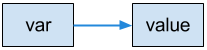
\includegraphics[height=25px]{pointer1.png}
	\caption{Variable in original program.}
	\label{pointer:1}
  \end{subfigure}\begin{subfigure}{0.5\textwidth}
	\centering
	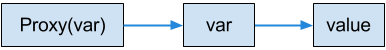
\includegraphics[height=25px]{pointer2.png}
	\caption{Proxied variable representation.}
	\label{pointer:2}
  \end{subfigure}
  \caption{Representation of a normal vs. proxied variable.}
\end{figure}

This is accomplished via Ruby's built-in \texttt{coerce} and \texttt{method\_missing} classes.  These methods are part of the Ruby language and implementation and are called on a variable if it does not have particular properties.  By overriding these functions, we can catch method calls using the proxied variable and store the variable information, argument, and function at the time of call to pass on to the SMT solver.\\

Specifically, \texttt{method\_missing} is called on the object if the object does not have a particular method defined, passing in the information for the original function call.  The default behavior of the Ruby interpreter is to simply raise an exception.\\

When an object that has been passed as an argument to another method which requires a specific type, but the object does not have a defined conversion to that type, the \texttt{coerce} method is called on that object.  If no suitable conversion is found, an exception will be raised.\\

\subsection{Z3}
Z3 is a SMT solver developed and released by Microsoft.  We use the Z3 programming API check satisfiability of the environment given a set of symbolic variables and contstraints.  This allows us to check whether or not it is possible for an assertion to fail at a certain point within a program.

\section{Implementation}
There are two main components of our implementation: the Z3 API and the proxy class for variables.

We have implemented proxy classes for both Ruby Fixnums and Booleans.

\section{Assessment}
using short ruby programs, see appendix

\section{Conclusion}
Summary and Future Work
More types of variables

\begin{thebibliography}{99}
\bibitem{rails}
A. Chaudhuri and J. Foster, ``Symbolic Security Analysis of Ruby-on-Rails Web Applications,'' in Proceedings of the 17th ACM Conference on Computer and Comm. Security, 2010, pp. 585-594.

\bibitem{typeinf}
B. Ren, J. Toman, T. S. Strickland, J. Foster, ``The Ruby Type Checker,'' in SAC '13: Proceedings of the 28th Annual ACM Symposium on Applied Computing, 2013.

\end{thebibliography}

\appendix
\section{Program 1}
\begin{verbatim}
Code goes here
\end{verbatim}

\end{document}
